\section{Metodologia Proposta}

\begin{slide}{Visão Geral dos Procedimentos}
  \centering
  \resizebox{0.9\textwidth}{!}{%
  \begin{tikzpicture}[
      every node/.style={font=\footnotesize},
      stage/.style={rectangle, rounded corners, draw=poliBlue, thick, align=center,
                    minimum width=2cm, minimum height=0.65cm, fill=blue!6},
      arrow/.style={->, thick, >=stealth},
      darrow/.style={->, thick, >=stealth, dashed},
      detail/.style={rectangle, rounded corners, draw=black!40, thick, align=center, font=\tiny, minimum width=2.2cm, minimum height=0.4cm, fill=gray!6},
    ]
    % Row 1
    \node[stage] (dados)      {Dados\\Experimentais};
    \node[stage, right=0.35cm of dados] (prep)  {Preparação\\dos Dados};
    \node[detail, below=0.1cm of prep, font=\tiny, draw=black!40, thick, minimum width=1.8cm, minimum height=0.35cm] {Z-score};
    \node[stage, right=0.35cm of prep] (eda)    {Análise\\Exploratória};
    \node[stage, right=0.35cm of eda] (sel) {Validação e\\Seleção};
    \draw[arrow] (dados) -- (prep);
    \draw[arrow] (prep) -- (eda);
    \draw[arrow] (eda) -- (sel);


    % Row 2
    \node[stage, below=0.9cm of sel] (fisico) {Modelo\\Físico 0D};
    \node[stage, right=0.35cm of fisico] (s0)    {Stage 0\\Clássicos};
    \node[stage, right=0.35cm of s0] (s1)    {Stage 1\\Redes Neurais};
    \node[stage, right=0.35cm of s1] (s2)    {Stage 2\\Híbridos};
    \draw[arrow] (fisico) -- (s0);
    \draw[arrow] (s0) -- (s1);
    \draw[arrow] (s1) -- (s2);
    % Connection Row1 -> Row2
    \draw[darrow] (sel.south) -- ++(0,-0.1) -| (fisico.north);

    % Row 3
    \node[stage, below=0.9cm of s2] (final) {Selecionado\\vs 0D};
    \draw[arrow] (s2) -- (final);

    % Connection Row2 -> Row3
    \draw[darrow] (s2.south) -- (final.north);
  \end{tikzpicture}
  }
  \note{Visão geral dos procedimentos: dados, preparação, análise exploratória, modelo físico 0D, Stage 0 (clássicos), Stage 1 (redes neurais), Stage 2 (híbridos), seleção pelo critério 1-SE e comparação final. [~1,5 min]}
\end{slide}
\begin{slide}{Etapa 1: Dados Experimentais}
  \small
  \begin{columns}
    \begin{column}{.35\linewidth}
      \begin{Item}
        \item 174 pontos experimentais do sistema V-AGMD piloto (LabMEMS/COPPE) \cite{curcino2023,Lisboa2024}
        \item 3 regimes de salinidade: 10, 40 e 70 g/L de NaCl
        \item 5 entradas: T$_{in,alim}$, T$_{in,ref}$, vazão$_{ref}$, P$_{vac}$, C$_{NaCl}$
        \item 3 saídas: Fluxo de permeado, T$_{out,alim}$, T$_{out,ref}$
      \end{Item}
      \vfill
      {\scriptsize Fonte dos dados: \cite{curcino2023,Lisboa2024}}
    \end{column}
    \begin{column}{.65\linewidth}
      \centering
      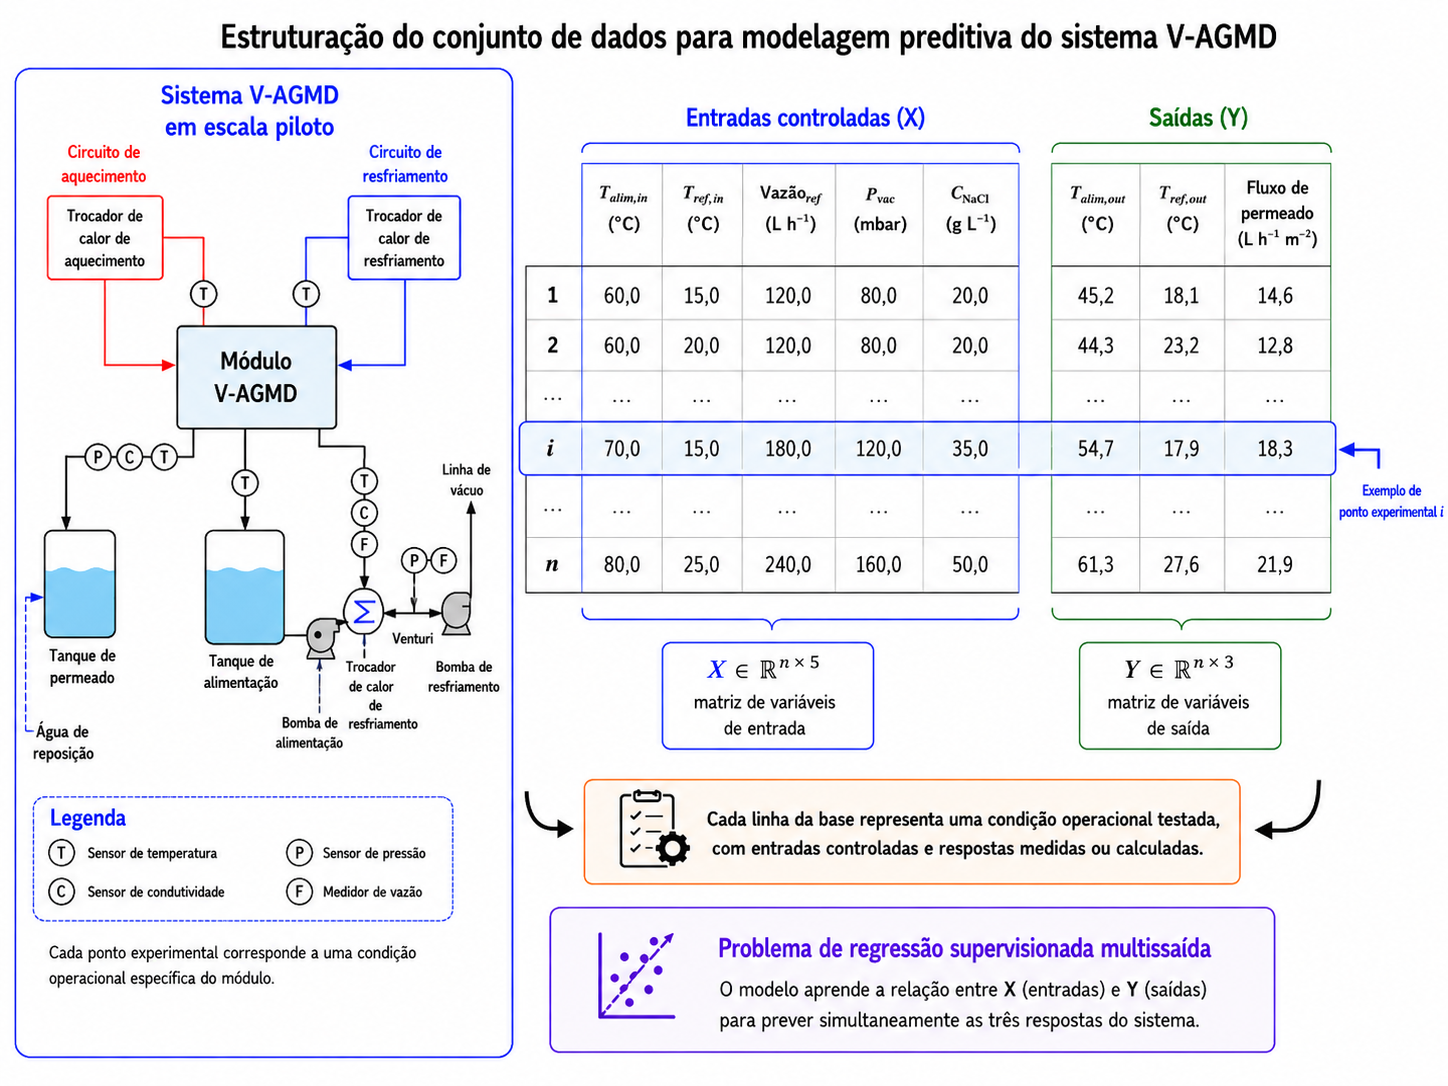
\includegraphics[width=\linewidth]{tcc_images/chap04/esquematizacao_regressao.png}
    \end{column}
  \end{columns}
  \note{O conjunto de dados tem 174 pontos experimentais obtidos em um sistema V-AGMD piloto, disponibilizado por Curcino et al. (2023) e Lisboa et al. (2024). Foram testados 3 regimes de salinidade: 10, 40 e 70 g/L. As 5 variáveis de entrada incluem temperaturas, vazão, pressão de vácuo e concentração salina. As 3 saídas são o fluxo de permeado e as duas temperaturas de saída. [~1 min]}
\end{slide}
\begin{slide}{Resumo — Decisões da Preparação dos Dados}
  \centering
  \small
  \begin{tabular}{lcp{7.5cm}}
    \rowcolor{poliBlue!20}
    \textbf{Etapa} & \textbf{Decisão} & \textbf{Justificativa} \\ \hline
    \rowcolor{gray!10}
    2.1 — Escalonamento & Z-score &
    Preserva a distribuição original dos dados; mede cada ponto em desvios-padrão, evitando compressão artificial na presença de valores extremos \\
    \rowcolor{white}
    2.2 — Validação & GroupKFold &
    Separa os folds por regime operacional, orientando a busca de hiperparâmetros para capacidade de \textbf{extrapolação} — diferente do KFold comum, que só avalia interpolação \\
  \end{tabular}
  \note{Slide de consolidação: resume as decisões de preparação dos dados e suas justificativas. [~1 min]}
\end{slide}
%========================================================================

\begin{slide}{Busca de Hiperparâmetros}
  \centering
  \small
  \begin{Item}
    \item Para cada família de modelos e cada \textbf{variável de saída} (target), foi realizado um ajuste independente de hiperparâmetros
    \item \textbf{Redes Neurais (MLP/Keras)}: \textbf{Random Search} (amostragem aleatória da grade) — maior espaço de busca (arquitetura, taxa de aprendizado, regularização)
    \item \textbf{Demais famílias} (lineares, árvores, híbridos): \textbf{busca exaustiva} (GridSearchCV) — espaço menor de hiperparâmetros
    \item Híbridos residuais: busca restrita (apenas regularização L2) para isolar o efeito da incorporação da física
  \end{Item}
  \vfill
  {\scriptsize \textbf{Legenda de cores:} \textcolor{blue!70!black}{azul} = modelos lineares \; \textcolor{green!70!black}{verde} = árvores de decisão \; \textcolor{orange!70!black}{laranja} = redes neurais \; \textcolor{red!70!black}{vermelho} = modelos híbridos (física + dados)}
  \note{A busca de hiperparâmetros foi feita por família e por target. Redes neurais usaram Random Search (espaço maior); as demais famílias usaram busca exaustiva. Híbridos residuais tiveram busca restrita (só L2). [~1,5 min]}
\end{slide}
%========================================================================

\begin{frame}
  \centering
  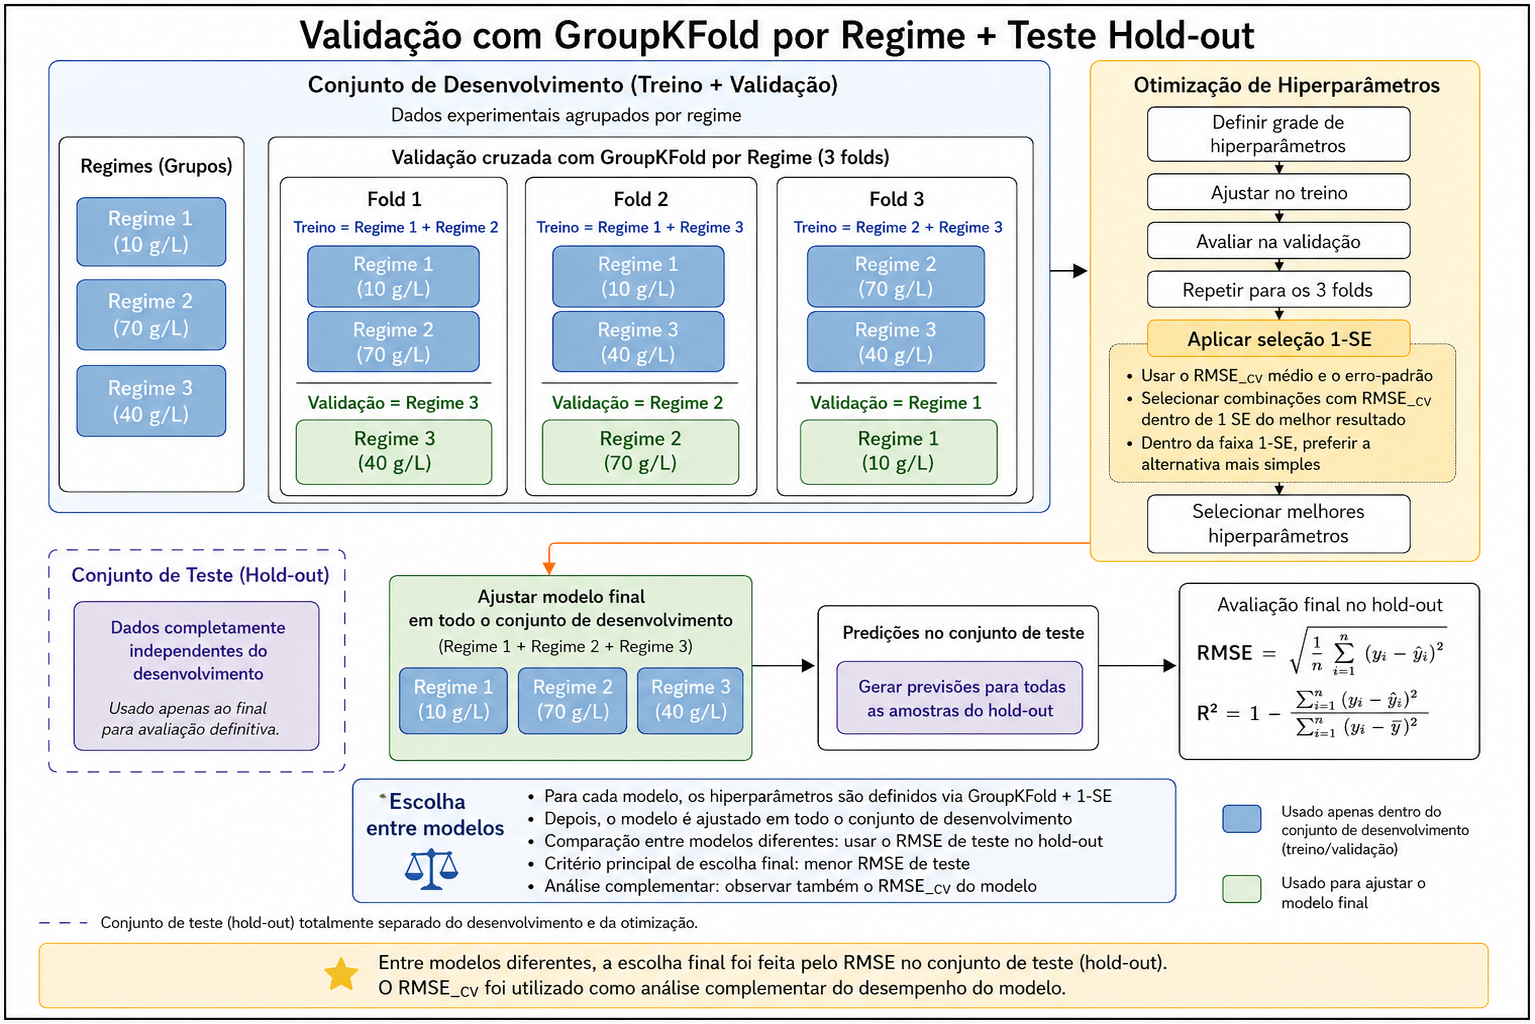
\includegraphics[width=0.75\linewidth]{tcc_images/chap04/criterio_selecao_esquema.png}
  \vfill
  {\scriptsize Fonte: Autor}
  \note{O fluxo completo: GroupKFold por regimes $\rightarrow$ RMSE$_{CV}$ m�dio com erro padr�o $\rightarrow$ regra 1-SE $\rightarrow$ sele��o do modelo mais simples dentro de 1 erro padr�o do melhor. [~1 min]}
\end{frame}

